
\subsubsection{Objective}
This research question investigates whether long-term temperature trends differ by elevation. To illustrate the phenomenon of elevation-dependent warming, this section focuses specifically on the highest elevation category: \textbf{2000+\,m (High Alpine)}.

\subsubsection{Methodology}
Using Apache Spark, monthly average temperature values (\texttt{tl\_mittel}) from the full dataset \texttt{climate\_all\_stations} were grouped by station and year. Station metadata was joined and used to classify each station into one of five predefined elevation bands:
    \begin{itemize}
      \item 0--499\,m (Lowland)
      \item 500--999\,m (Upland)
      \item 1000--1499\,m (Lower Alps)
      \item 1500--1999\,m (Alpine)
      \item 2000+\,m (High Alpine)
    \end{itemize}
    
Two additional plots were generated for context:
\begin{itemize}
    \item A distribution plot of all stations by elevation zone and region.
    \item A labeled diagram of the highest station per region to confirm extreme values.
\end{itemize}

\subsubsection{Results and Interpretation}

\paragraph{Figure~\ref{fig:temptrend_highalpine}: Temperature Trends in the High Alpine Zone}
The line plot below shows annual average temperatures from 1970 to 2025 for each region in the High Alpine zone. A general increase is evident. The curves show irregularities, stagnation phases, and sudden drops—indicating either microclimatic variability or data limitations.

In addition, abrupt changes and missing values are visible at several lines. These are most likely caused by:
\begin{itemize}
    \item sensor malfunctions,
    \item missing or incomplete historical data,
    \item or gaps due to station shutdowns.
\end{itemize}
These patterns emphasize the importance of pairing trend analysis with a careful check of data completeness.

\begin{figure}[ht]
  \centering
    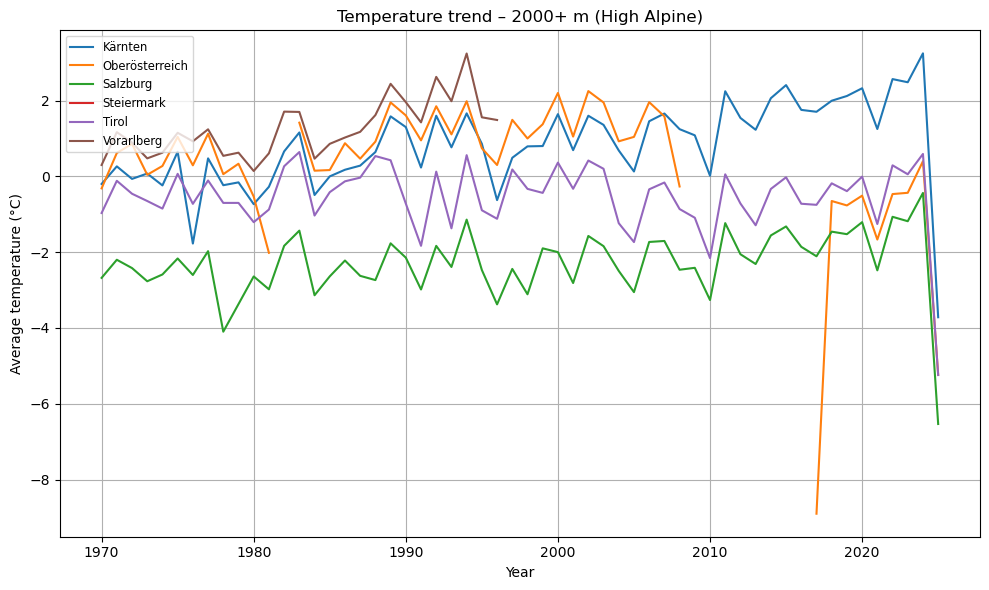
\includegraphics[width=0.45\textwidth]{img/temptrend_highalpine.png}
  \caption{Average annual temperature trends (1970–2025) in 2000+ High Alpine zone}
    \label{fig:temptrend_highalpine}
\end{figure}

\paragraph{Figure~\ref{fig:station_distribution_highalpine}: Altitude Distribution of Weather Stations}
This scatterplot validates that stations assigned to the High Alpine zone are located well above 2000+. The distribution also shows regional diversity, which supports cross-regional comparisons.

\begin{figure}[ht]
    \centering
    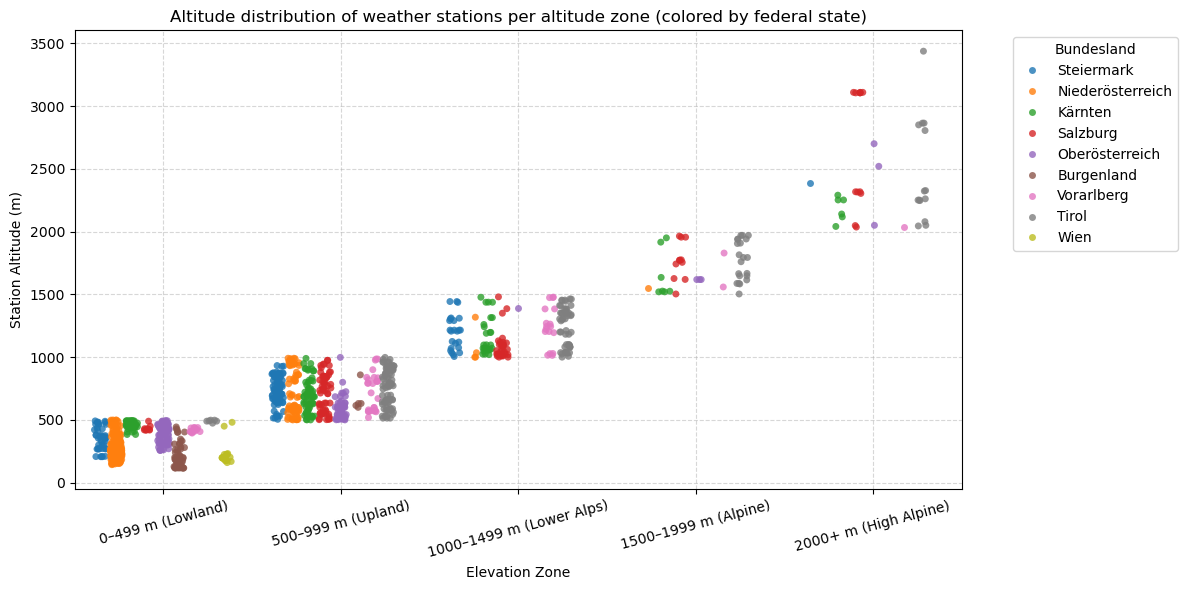
\includegraphics[width=0.45\textwidth]{img/station_distribution_highalpine.png}
    \caption{Elevation distribution of stations by zone and region}
    \label{fig:station_distribution_highalpine}
\end{figure}

\paragraph{Figure~\ref{fig:highest_stations_labeled}: Highest Stations per Region}
This annotated graphic confirms the locations and altitudes of the weather stations in the two highest altitude zones per federal state.

\begin{figure}[ht]
    \centering
    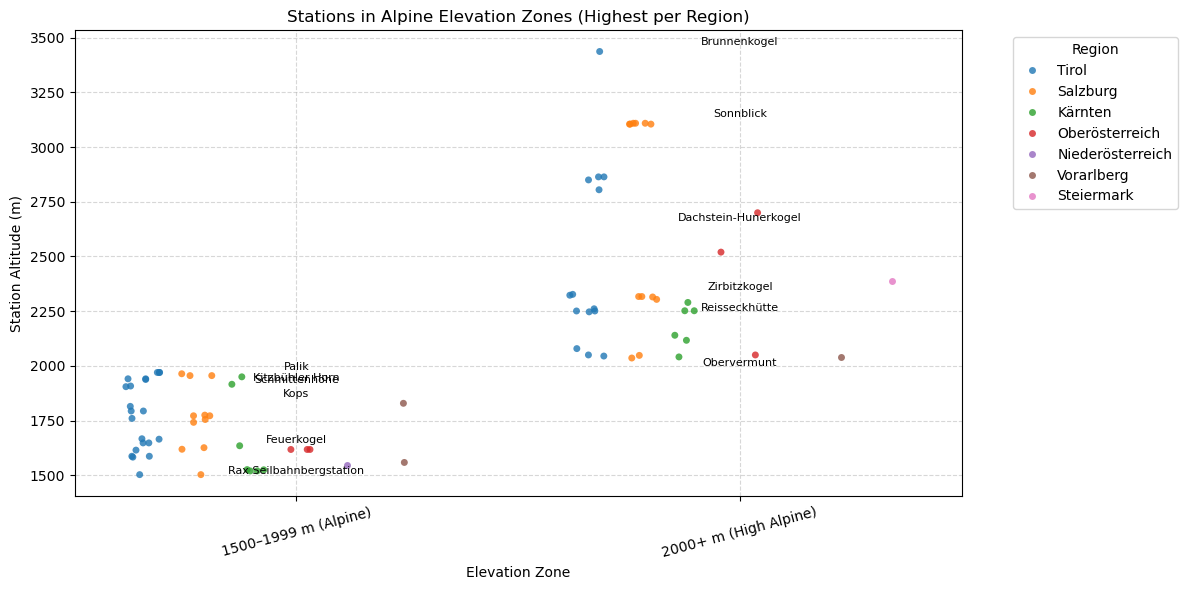
\includegraphics[width=0.45\textwidth]{img/highest_stations_labeled.png}
    \caption{Highest station per region in Alpine zones with labels}
    \label{fig:highest_stations_labeled}
\end{figure}

\subsubsection{Conclusion}
The high alpine zone (2000+) in Austria shows a clear warming trend over the last five decades. Regional fluctuations are present, but do not affect the overall pattern. Exactly the same analysis was carried out for the four lower altitude zones; these analyses are included in the Jupyter Notebook.
